\begin{problem}{타일 뒤집기(Hard)}{standard input}{standard output}

석환이는 신기한 게임판을 가지고 있다. 이 게임판에는 한 면은 검은색, 한 면은 흰색으로 칠해진 타일이 $N$행 $N$열으로 배치되어 있다. 각 타일은 제자리에서 뒤집을 수 있는데, 타일 하나를 뒤집으면 그 타일과 상하좌우로 인접한 타일들이 같이 뒤집힌다. 석환이는 타일들이 무작위로 배치된 게임판에서 타일들을 적당히 뒤집어서 모든 타일이 흰색 면이 위를 향하도록 만드는 놀이를 좋아한다.

\begin{center}
  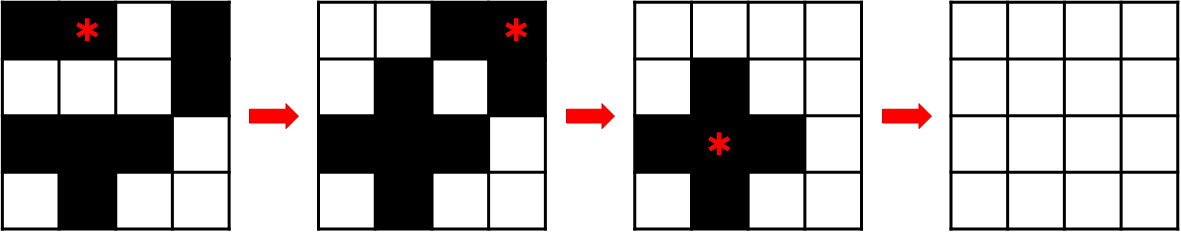
\includegraphics[width=0.8\textwidth]{tile1.png}
\end{center}

어느 날, 석환이가 게임판을 가지고 놀다가 자리를 비운 사이 석환이의 동생이 이 게임판을 발견했다. 석환이의 동생은 놀이의 규칙을 모르기 때문에, 그냥 처음 상태에서 검은색 면이 위를 향하고 있는 타일들을 전부 한 번씩 뒤집어 보았다. 그러자 놀랍게도 모든 타일이 흰색 면이 위를 향하게 되었다!

\begin{center}
  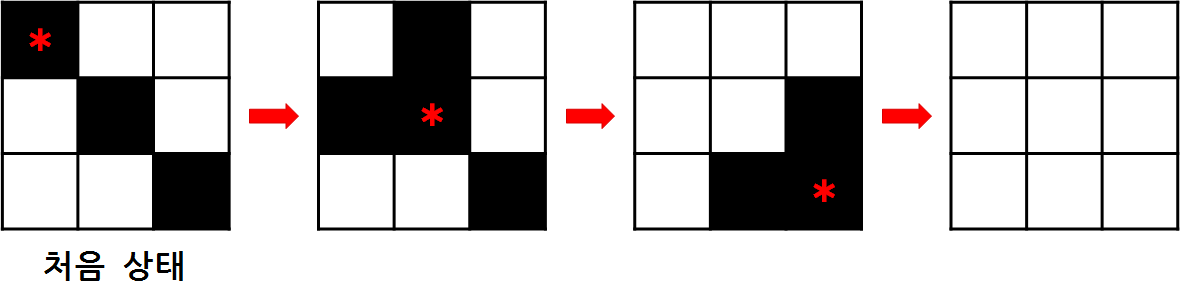
\includegraphics[width=0.8\textwidth]{tile2.png}
\end{center}

돌아온 석환이는 동생에게 놀이의 규칙을 알려 주려고 했지만, 그 전에 동생이 즐거워하는 모습을 더 보고 싶어져서 같은 특징을 갖는 게임판을 몇 번 더 만들어 주기로 했다. 석환이는 멋진 해커이기 때문에 게임판의 규칙을 따르지 않고 타일을 하나씩만 뒤집을 수도 있다. 하지만 아무 조건 없이 타일을 뒤집는 것은 별로 재미가 없었기 때문에, 석환이는 게임판에서 몇 개의 타일들은 뒤집지 않고 원하는 배치를 만들어 보기로 했다.

\InputFile
첫 번째 줄에 게임판의 크기 $N$($1 \le N \le 1,000$)이 주어진다.

두 번째 줄부터 $N$개의 줄에 걸쳐 게임판의 타일들의 상태를 나타내는 $N$글자의 문자열이 주어진다. 문자열은 \texttt{\#}와 \texttt{.}, \texttt{-}만으로 이루어져 있으며, \texttt{\#}는 검은색 면이 위를 향하도록 고정된 타일, \texttt{.}는 흰색 면이 위를 향하도록 고정된  타일, \texttt{-}는 석환이가 마음대로 뒤집을 수 있는 타일을 의미한다.

\OutputFile
$N$개의 줄에 걸쳐 석환이의 동생이 검은색 면이 위를 향하고 있는 타일들을 전부 한 번씩 뒤집어서 모든 타일이 흰색 면이 위를 향하도록 만들 수 있는 게임판의 모양을 출력한다. 입력 조건과 마찬가지로 검은색 면이 위를 향하고 있는 타일은 \texttt{\#}, 흰색 면이 위를 향하고 있는 타일은 \texttt{.}로 나타낸다.

답이 여러 가지일 경우 아무것이나 출력하고, 답이 존재하지 않을 경우 \texttt{thinking\_face}를 출력한다.

\Example

\begin{example}
\exmp{7
---.---
-----.-
--\#----
.------
------\#
-.-----
----\#--}{\#.\#.\#\#\#
....\#.\#
\#.\#\#\#\#\#
..\#.\#..
\#\#\#\#\#.\#
\#.\#....
\#\#\#.\#.\#}%
\exmp{5
----\#
\#--.-
-\#---
----.
--.--}{thinking\_face}%
\end{example}

\end{problem}
